\textbf{Pour cette première partie, aucune justification n'est demandée et une seule réponse est possible par question. Pour chaque question, reportez son numéro sur votre copie et indiquez votre réponse.}

\subsubsection*{Question 1}
L'inverse du double de 5 est égal à :

\textbf{a.} $\dfrac{1}{10}$\hfill \textbf{b.} $\dfrac{1}{5}$\hfill \textbf{c.} $\dfrac{5}{2}$\hfill \textbf{d.} 10

\subsubsection*{Question 2}
On considère la relation $F = a + \dfrac{b}{cd}$.

Lorsque $a = \dfrac{1}{2}$, $b = 3$, $c = 4$, $d = -\dfrac{1}{4}$, la valeur de $F$ est égale à :

\textbf{a.} $-\dfrac{5}{2}$\hfill \textbf{b.} $-\dfrac{3}{2}$\hfill \textbf{c.} $\dfrac{5}{2}$\hfill \textbf{d.} $\dfrac{3}{2}$

\subsubsection*{Question 3}
Le prix d'un article est multiplié par 0,975.

Cela signifie que le prix de cet article a connu :

\textbf{a.}  une baisse de 2,5\% \hfill \textbf{b.} une augmentation de 97,5\%

\textbf{c.} une baisse de 25\%\hfill \textbf{d.} une augmentation de 0,975\%

\subsubsection*{Question 4}
Le prix d'un article est noté $P$. Ce prix augmente de 10\% puis baisse de 10\%.

À l'issue de ces deux variations, le nouveau prix est noté $P_1$. On peut affirmer que :

\textbf{a.} $P_1 = P$\hfill \textbf{b.} $P_1 > P$\hfill \textbf{c.} $P_1 < P$\hfill \textbf{d.} Cela dépend de $P$

\subsubsection*{Question 5}
On lance un dé à 4 faces. La probabilité d'obtenir chacune des faces est donnée dans le tableau ci-dessous :

\begin{center}
\begin{tabular}{|c|c|c|c|}
\hline
Face numéro 1 & Face numéro 2 & Face numéro 3 & Face numéro 4 \\
\hline
0,5 & $\dfrac{1}{6}$ & 0,2 & $x$ \\
\hline
\end{tabular}
\end{center}

On peut affirmer que :

\textbf{a.} $x = \dfrac{2}{15}$\hfill \textbf{b.} $x = \dfrac{2}{3}$\hfill \textbf{c.} $x = 0,4$\hfill \textbf{d.} $x = 0,1$

\subsubsection*{Question 6}
On considère $x,~y~\text{et}~u$ des réels non nuls tels que $\dfrac{1}{x} + \dfrac{1}{y} = \dfrac{1}{u}.$

On peut affirmer que :

\textbf{a.} $u = \dfrac{xy}{x+y}$\hfill \textbf{b.} $u = \dfrac{x+y}{xy}$\hfill \textbf{c.} $u = xy$\hfill \textbf{d.} $u = x+y$

\subsubsection*{Question 7}

\begin{minipage}[t]{0.6\textwidth}
On a représenté ci-contre la parabole d'équation $y = x^2$.

On note ($J$) l'inéquation, sur $\mathbb{R}$, $x^2 \geq 10$.

\smallskip

L'inéquation ($J$) est équivalente à :

\smallskip

\textbf{a.} $-\sqrt{10} \leq x \leq \sqrt{10}$\hfill \textbf{b.} $x \leq -\sqrt{10}$ ou $x \geq \sqrt{10}$

\smallskip

\textbf{c.} $x \geq \sqrt{10}$\hfill \textbf{d.} $x = \sqrt{10}$ ou $x = -\sqrt{10}$
\end{minipage}
\hfill
\begin{minipage}[t]{0.35\textwidth}
\vspace{0pt}
\begin{center}
  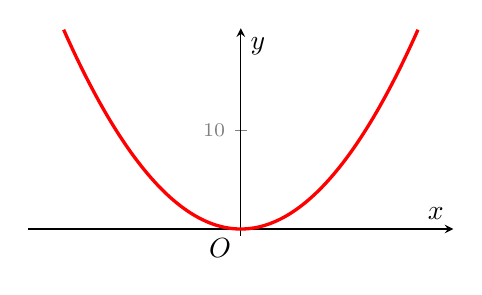
\begin{tikzpicture}[declare function={f(\x) = \x^2;}]
    \begin{axis}[
        clip=false,
        axis y line=center,axis x line=middle,
        x=0.5cm,y=0.125cm,
        xmin=-5.4,xmax=5.4,ymin=-0.7,ymax=20.4,
        xtick =\empty,ytick ={10},
        grid=none,
        tick label style={font=\scriptsize,black!50},
        xlabel=$x$,ylabel=$y$
      ]
      \addplot[mark=none,red,very thick,domain=-4.5:4.5,samples=150] {f(x)};
      \coordinate[label={below left=1mm}:$O$] (O) at (0, 0);
    \end{axis}
  \end{tikzpicture}
\end{center}
\end{minipage}

\subsubsection*{Question 8}

\begin{minipage}[t]{0.6\textwidth}
On a représenté ci-contre une droite $D$ dans un repère orthonormé. Une équation de la droite $D$ est :

\bigskip

\textbf{a.} $y = -\dfrac{3}{2}x + 2$\hfill \textbf{b.} $y = \dfrac{2}{3}x + 2$

\bigskip

\textbf{c.} $2x - 3y - 6 = 0$\hfill \textbf{d.} $\dfrac{x}{3} + \dfrac{y}{2} - 1 = 0$
\end{minipage}
\hfill
\begin{minipage}[t]{0.35\textwidth}
\vspace{0pt}
\begin{center}
  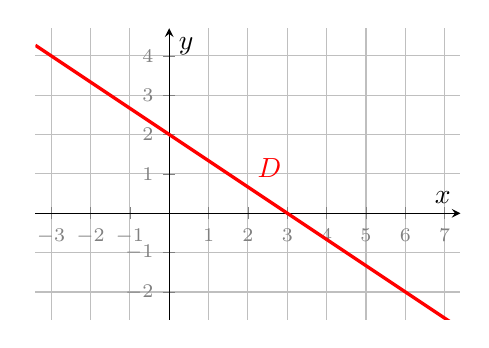
\begin{tikzpicture}[declare function={f(\x) = -2/3*\x+2;}]
    \begin{axis}[
        axis y line=center,axis x line=middle,
        x=0.5cm,y=0.5cm,
        xmin=-3.4,xmax=7.4,ymin=-2.7,ymax=4.7,
        xtick distance = 1,ytick distance = 1,
        grid=major,
        tick label style={font=\scriptsize,black!50},
        xlabel=$x$,ylabel=$y$
      ]
      \addplot[mark=none,red,very thick,domain=-3.4:7.4,samples=150] {f(x)};
      \addplot[mark=none,only marks,samples at={2},red,nodes near coords=$D$,nodes near coords style={anchor={south west}}] {f(x)};
    \end{axis}
  \end{tikzpicture}
\end{center}
\end{minipage}

\subsubsection*{Question 9}
On considère trois fonctions définies sur $\mathbb{R}$ :

$f_1 : x \mapsto x^2 - (1 - x)^2$\hfill $f_2 : x \mapsto \dfrac{x}{2} - \left(1 + \dfrac{1}{\sqrt{2}}\right)$\hfill $f_3 : x \mapsto \dfrac{5 - \dfrac{2}{3}x}{0,7}$

Parmi ces trois fonctions, celles qui sont des fonctions affines sont :

\textbf{a.} aucune\hfill \textbf{b.} toutes

\textbf{c.} uniquement la fonction $f_1$\hfill \textbf{d.} uniquement les fonctions $f_2$ et $f_3$

\subsubsection*{Question 10}

\begin{minipage}[t]{0.6\textwidth}
On a représenté ci-contre une parabole $P$.

Une seule des quatre fonctions ci-dessous est susceptible d'être représentée par la parabole $P$.

Laquelle ?

\smallskip

\textbf{a.} $x \mapsto x^2 - 10$\hfill \textbf{b.} $x \mapsto -x^2 - 10$

\smallskip

\textbf{c.} $x \mapsto -x^2 + 10$\hfill \textbf{d.} $x \mapsto -x^2 + 10x$
\end{minipage}
\hfill
\begin{minipage}[t]{0.35\textwidth}
\vspace{0pt}
\begin{center}
  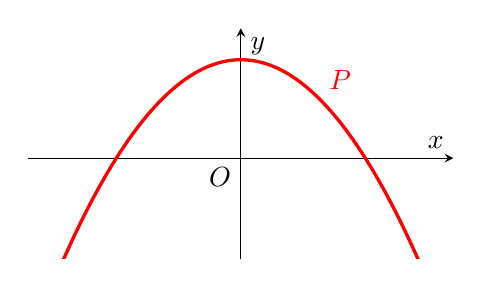
\begin{tikzpicture}[declare function={f(\x) = -\x^2 + 10;}]
    \begin{axis}[
        axis y line=center,axis x line=middle,
        x=0.5cm,y=0.125cm,
        xmin=-5.4,xmax=5.4,ymin=-10.2,ymax=13.2,
        xtick =\empty,ytick = \empty,
        grid=none,
        tick label style={font=\scriptsize,black!50},
        xlabel=$x$,ylabel=$y$
      ]
      \addplot[mark=none,red,very thick,domain=-5.4:5.4,samples=150] {f(x)};
      \coordinate[label={below left=1mm}:$O$] (O) at (0, 0);
      \addplot[mark=none,only marks,samples at={2},red,nodes near coords=$P$,nodes near coords style={anchor={south west}}] {f(x)};
    \end{axis}
  \end{tikzpicture}
\end{center}
\end{minipage}

\subsubsection*{Question 11}

\begin{minipage}[t]{0.6\textwidth}
On a représenté ci-contre la courbe $C$ d'une fonction $f$.

\smallskip

Les points A, B, R et S appartiennent à la courbe $C$.

\smallskip

Leurs abscisses sont notées respectivement $x_A, x_B, x_R$ et $x_S$.

\smallskip

L'inéquation $x \times f(x) > 0$ est vérifiée par :
\end{minipage}
\hfill
\begin{minipage}[t]{0.35\textwidth}
\vspace{0pt}
\begin{center}
  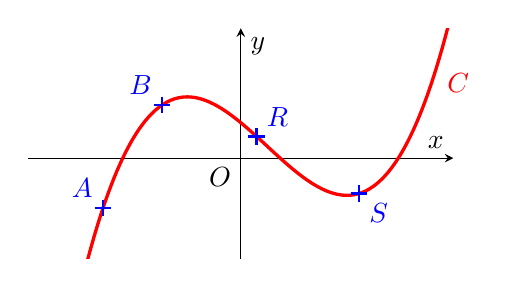
\begin{tikzpicture}[declare function={f(\x) = 0.3*(\x - 4) * (\x - 1) * (\x +3);}]
    \begin{axis}[
        axis y line=center,axis x line=middle,
        x=0.5cm,y=0.125cm,
        xmin=-5.4,xmax=5.4,ymin=-10.2,ymax=13.2,
        xtick =\empty,ytick = \empty,
        grid=none,
        tick label style={font=\scriptsize,black!50},
        xlabel=$x$,ylabel=$y$
      ]
      \addplot[mark=none,red,very thick,domain=-5.4:5.4,samples=150] {f(x)};
      \coordinate[label={below left=1mm}:$O$] (O) at (0, 0);
      \addplot[mark=none,only marks,samples at={5},red,nodes near coords=$C$,nodes near coords style={anchor={north west}}] {f(x)};
      \addplot[mark=+,mark size=3pt,thick,only marks,blue,nodes near coords={$A$},nodes near coords style={anchor=south east},samples at={-3.5}]{f(x)};
\addplot[mark=+,mark size=3pt,thick,only marks,blue,nodes near coords={$B$},nodes near coords style={anchor=south east},samples at={-2}]{f(x)};
\addplot[mark=+,mark size=3pt,thick,only marks,blue,nodes near coords={$R$},nodes near coords style={anchor=south west},samples at={0.4}]{f(x)};
\addplot[mark=+,mark size=3pt,thick,only marks,blue,nodes near coords={$S$},nodes near coords style={anchor=north west},samples at={3}]{f(x)};
\end{axis}
  \end{tikzpicture}
\end{center}
\end{minipage}

\smallskip

\textbf{a.} $x_A$ et $x_B$\hfill \textbf{b.} $x_A$ et $x_R$

\textbf{c.} $x_A$ et $x_S$\hfill \textbf{d.} $x_A, x_B$ et $x_S$

\subsubsection*{Question 12}
Voici une série de notes avec les coefficients associés.

\begin{center}
\begin{tabular}{|c|c|c|c|}
\hline
Note & 10 & 8 & 16 \\
\hline
Coefficient & 1 & 2 & $x$ \\
\hline
\end{tabular}
\end{center}

On note $m$ la moyenne de cette série. Que doit valoir $x$ pour que $m = 15$ ?

\textbf{a.} impossible\hfill \textbf{b.} $x = 10^{-3}$

\textbf{c.} $x = 3$\hfill \textbf{d.} $x = 19$
